\documentclass{article}
%\usepackage[utf8]{inputenc}
\usepackage{graphicx, amsmath,amssymb,latexsym, booktabs,array,multirow}
\usepackage{listings}
\usepackage{flexisym}
\usepackage{graphicx}
%\usepackage[]{mcode}
\usepackage
[
        a4paper,% other options: a3paper, a5paper, etc
        left=2.54cm,
        right=2.54cm,
        top=1.5cm,
        bottom=1.8cm,
        % use vmargin=2cm to make vertical margins equal to 2cm.
        % us  hmargin=3cm to make horizontal margins equal to 3cm.
        % use margin=3cm to make all margins  equal to 3cm.
]{geometry}
\DeclareMathOperator*{\argmax}{argmax}
\title{Data Visualisation}
\author{ankitamehta }
\date{March 2017}

\usepackage{natbib}
\usepackage{hyperref}
\usepackage{graphicx}
\usepackage{tikz}
\begin{document}

\hrule height 1pt
\vspace{1em}
\begin{center}
\large{Reinforement Learning(687) - Assignment 1 }\\
\large{Submitted by : Ankita Mehta }\\
\end{center}
\par
\section*{Part One:}

\subsection*{Question 1:}
Given an MDP  \(M = (S, A, P, R, d_0, \gamma)\)  and a fixed policy, $\pi$ , the probability that the action at time \(t=0\)  is a $\in$ A is: \[Pr(a_0 = a) = \sum_{s \in S}d_0(s)\pi(s,a)\]
Write similar expressions (using only the terms defined in M) for the following:

\begin{enumerate}
\item The probability that the state at time \(t=3\) is either s $\in$ S or $s\textprime$ $\in$ S: \\

\begin{align}
Pr (S_3 = s) = &\sum_{\substack {s_2 \in S \\ a_2 \in A}} Pr(S_3 = s | S_2 = s_2 , A_2 = a_2) * Pr(S_2 = s_2 , A_2 = a_2) \nonumber \\
                     = &\sum_{\substack {s_2 \in S \\ a_2 \in A}}P(s_2,a_2,s) * Pr(A_2 = a_2 | S_2 = s_2) * Pr(S_2 = s_2) \nonumber  \\
                     = &\sum_{\substack {s_2 \in S \\ a_2 \in A}}P(s_2,a_2,s) * \pi(s_2,a_2) * Pr(S_2 = s_2) 
\end{align}

Propagating equation 1 backwards till it reaches $s_0$, and then approaching same way when s = s\textprime , we get the following equation : \\
\[Pr(S_3 = s|s\textprime) = \sum\limits_{\substack{s_2,s_1,s_0 \in S\\ a_2,a_1,a_0  \in A}}P(s_2, a_2,s)*\pi(s_2, a_2)*P(s_1, a_1,s_2)*\pi(s_1,a_1)*P(s_0,a_0,s_1)*\pi(s_0,a_0).d_0(s_0)\] 
\[ + \sum\limits_{\substack{s_2,s_1,s_0 \in S\\ a_2,a_1,a_0  \in A}}P(s_2, a_2,s\textprime)*\pi(s_2, a_2)*P(s_1, a_1,s_2)*\pi(s_1,a_1)*P(s_0,a_0,s_1)*\pi(s_0,a_0).d_0(s_0)\] 

\item The probability that the action at time \(t = 16\) is a\textprime $\in$ A given that the action at time \(t = 15\) is a $\in$  A and the state at time \(t = 14\) is s:

\[Pr(A_{16} = a\textprime | A_{15} = a , S_{14} = s) = \sum\limits_{\substack{s_{15},s_{16} \in S\\ a_{14}  \in A}} \pi(s_{16},a\textprime)*P(s_{15},a, s_{16})*P(s, a_{14},s_{15})*\pi(s, a_{14})\]

\item The expected reward at time \(t=6\) given that the action at time \(t=3\) is a $\in$ A, and the state at time \(t=5\) is s $\in$ S:

\[\mathbb{E}(R_6 | A_3 = a, S_5 = s) =  \sum\limits_{\substack{s_6,s_7 \in S\\ a_6,a_5 \in A}} R(s_6,a_6,s_7)*P(s_6, a_6, s_7)*\pi(s_6,a_6)*P(s, a_5, s_6)*\pi(s, a_5)\]

\item The probability that the initial state was s $\in$ S given that the state at time \(t=1\) is s\textprime $\in$ S.

\[Pr(S_0 = s | S_1 = s\textprime) = \frac{Pr(S_0=s,S_1=s\textprime)} {Pr(S_1=s\textprime)}\] 

\begin{align}
Pr(S_0=s,S_1=s\textprime) &= \sum_{a \in A} Pr(S_1 = s\textprime | S_0 = s, A_0 = a) * Pr(A_0 = a | S_0 = s) * Pr(S_0 = s)\nonumber \\
                                              &= \sum_{a \in A} P(s, a, s\textprime) * \pi(s, a) * d_0(s)
\end{align}

\begin{align}
Pr(S_1 = s\textprime) &=\sum\limits_{\substack{s \in S\\ a \in A}}Pr(S_1 = s\textprime | S_0 = s, A_0 = a) * Pr(S_0 = s , A_0 = a) \nonumber \\ 
                                    & = \sum\limits_{\substack{s \in S\\ a \in A}}P(s, a, s\textprime) * Pr(A_0 = a | S_0 = s) * Pr(S_0 = s) \nonumber \\
                                    & = \sum\limits_{\substack{s \in S\\ a \in A}}P(s, a, s\textprime) * \pi(s, a) * d_0(s)
\end{align}

From equation 1 and 2 , \[Pr(S_0 = s | S_1 = s\textprime) =\frac{\sum_{a \in A} P(s, a, s\textprime) * \pi(s, a) * d_0(s)}{\sum\limits_{\substack{s \in S\\ a \in A}}P(s, a, s\textprime) * \pi(s, a) * d_0(s)} \]

\item The probability that the action at time \(t = 5\) is a $\in$ A given that the initial state is s $\in$S, the state at time \(t=5\) is s\textprime $\in$S , and the action at time \(t=6\) is a\textprime $\in$ A.

\begin{align}
Pr(A_5 = a | S_0 = s , S_5 = s\textprime , A_6 = a\textprime)  & = \frac{Pr(A_5 = a, S_5 = s\textprime, A_6 = a\textprime)} {Pr(S_5 = s\textprime,A_6 = a\textprime)}									     
\end{align}

\begin{align}
Pr(A_5 = a, S_5 = s\textprime, A_6 = a\textprime) &= \sum\limits_{s\textprime\textprime \in S} Pr(A_6=a\textprime | S_6 = s\textprime\textprime) * Pr(S_6 = s\textprime\textprime |A_5 = a,S_5 = s\textprime) * Pr(A_5 = a | S_5 = s\textprime) \nonumber \\
									    &= \sum\limits_{s\textprime\textprime \in S} \pi(s\textprime\textprime, a\textprime) * P(s\textprime, a , s\textprime\textprime) * \pi(s\textprime , a)									
\end{align}

\begin{align}
Pr(S_5 = s\textprime,A_6 = a\textprime) &=\sum\limits_{s\textprime\textprime \in S} Pr(A_6 = a\textprime | S_6 = s\textprime\textprime) * \sum\limits_{a\in A} Pr(S_6 =s\textprime\textprime | S_5 = s\textprime, A_5 =a ) * Pr(A_5 = a | S_5 = s\textprime) \nonumber \\
							     &=\sum\limits_{s\textprime\textprime \in S} \pi(s\textprime\textprime , a\textprime)* \sum\limits_{a\in A} P(s\textprime , a , s\textprime\textprime) * \pi(s\textprime,a)
\end{align}

Putting equation 5 and 6 in 4 , we get:

\[ Pr(A_5 = a | S_0 = s , S_5 = s\textprime , A_6 = a\textprime) = \frac{\sum\limits_{s\textprime\textprime \in S} \pi(s\textprime\textprime, a\textprime) * P(s\textprime, a , s\textprime\textprime) * \pi(s\textprime , a)} {\sum\limits_{s\textprime\textprime \in S} \pi(s\textprime\textprime , a\textprime)* \sum\limits_{a\in A} P(s\textprime , a , s\textprime\textprime) * \pi(s\textprime,a)}\]

\end{enumerate}

\subsection*{Question 2:} How many deterministic policies are there for an MDP with \(|S| < \infty\) and \(|A| < \infty\) ? \\

\textbf{Solution:}  Number of possible deterministic policies for MDP with finite S and A are : $|A|^ {|S|}$. For example, lets consider S = {$s_1$, $s_2$,$s_3$} and A = {0,1}.  Possible deterministic policies with this state-action space are:
{0,0,0} ;  {0,0,1} ; {0,1,0} ; {0,1,1} ; {1,0,0} ; {1,0,1} ; {1,1,0} ; {1,1,1}, which are total 8.

\subsection*{Question 3:} In Pendulum Domain Problem, which of the two variant mentioned in question would require more episodes to solve ? \\

\textbf{Solution:} The variant where the initial angle is chosen randomly between [-$\pi$ , $\pi$] is expected to take more number of episodes to solve. This is because, with deterministic initial state pendulum always has to start from the fixed state $(0,0)$ whereas in stochastic one, its initial state is changing every time. Since the randomness of initial state has increased, so the agent will need more number of episodes to decide at which initial state, it has to provide how much amount of torque so that it reach the goal state within 20 sec.

\subsection*{Question 4:} How many episodes do you expect an agent should need in order to find near-optimal policies for the gridworld and pendulum domains?\\

\textbf{Solution:} If we plan to go by brute force method, i.e running the agent for all possible policies, then expected number of episodes for gridworld domain would be $4^ {23}$, i.e $|A|^ {|S|}$. Whereas in pendulum domain, since its state-action space is continuous so its not easy to quantify but it would be very large.

\subsection*{Question 5:} Select a problem that we have not talked about in class, where the agent does not fully observe the state. Describe how this problem can be formulated as an MDP ?\\

\textbf{Solution:} Let's consider the game of solitaire with 7 decks and 4 locations on top , in which the agent is playing the game. Goal of agent is to win the game. In this game, agent can only see the current cards but not all the cards, which makes it partially observable. 
We can formulate this problem as an MDP in following way: \\

\noindent
S = It is a huge space with every possible combination of cards on each deck and 4 specific locations. \\
A = pick and drop under other card , pick and drop on same location, pick and drop on upper 4 locations given, open the new card\\
P(s, a, s\textprime) = Next combination of cards on each deck, locations given the current combination of cards on each deck, locations and taken action a from A.\\
R = 1 , when it will win the game, otherwise 0\\
$\gamma = 1$ , because what it matters is agent should win the game.\\
$d_0$ = Any one card from the visible cards to the agent\\

\noindent
Here, in MDP all states are the part of environment. Whereas the agent can only see the open cards, so he will have to make an observation on how to process those cards to win the game. So that will be the part of agent not environment.

\section*{Part Two: Programming}
\subsection*{a: Code } 


$VectorXd  \quad temp;$\\
$MatrixXd  \quad sigma\_temp = MatrixXd::Zero(numParams, numParams);$\\
$theta.setZero();$\\
$Sigma = MatrixXd::Identity(numParams, numParams);$\\
$for (int \quad i = 0 ;\quad i < numElite; \quad i++ )$\\
 \{\\
 $\hspace*{2em} theta  \quad+= \quad thetas[i];$\\
 \}\\
$theta = theta / numElite;$\\
$for (int \quad i = 0 ;\quad i < numElite; \quad i++ )$\\
\{\\
$\hspace*{2em} temp = thetas[i] - theta;$\\
$\hspace*{2em} sigma\_temp \quad+= temp * (temp.transpose());$\\
\}\\
$Sigma \quad= (Sigma*100 + sigma\_temp ) / (numElite + 100);$\\

\subsection*{b: GridWorld Hyperparameters} Best hyperparameters found for Gridworld problem are : 
Population (K) : 10 \\
NumElite ($K_e$) : 3 \\
EpisodesPerPolicy (N) : 1 \\
sigma : 2.3 \\
epsilon : 100 \\
Plot of Episodes versus Expected return for this problem can be seen in Figure \ref{fig:grid} :\\

\subsection*{c: Pendulum deterministic Hyperparameters} Best hyperparameters found for Pendulum deterministic problem are :\\
Population (K) : 10 \\
NumElite ($K_e$) : 3 \\
EpisodesPerPolicy (N) : 1 \\
sigma : 2.3 \\
epsilon : 100 \\
Plot of Episodes versus Expected return for this problem can be seen in Figure \ref{fig:pendulum-D} :\\

\subsection*{d: Pendulum stochastic Hyperparameters} Best hyperparameters found for Pendulum Stochastic problem are : \\
Population (K) : 10 \\
NumElite ($K_e$) : 3 \\
EpisodesPerPolicy (N) : 8 \\
sigma : 2.3 \\
epsilon : 100 \\
Plot of Episodes versus Expected return for this problem can be seen in Figure \ref{fig:pendulum-S} :\\

\subsection*{e: CEM} Write a brief statement describing your experience getting CEM working.
\begin{enumerate}
\item How long did it take (wall-time) to get working?\\

Understanding the whole problem, writing the code and then performing Gridworld took almost 6-7 hours. But after that, it took 4-5 hours to generate the complete results.

\item Roughly how many times would you estimate you ran an agent for a full lifetime (multiple episodes starting from an initial policy) total on each domain?\\

In Gridworld, I ran an agent for 15 times with 5-10 trials each time. Then I ran the agent again for 3 times, each having 1000 trials. \\
In Pendulum Deterministic, I ran an agent for four times with 3-5 trials each time. Then I ran the agent again for 8 times, each having 100 trials.\\
In Pendulum Stochastic, I ran an agent for 3 times with 5-10 trials each time. Then I ran the agent again for 5 times, each having 30 trials.\\

Note: After running and observing all the experiments for each domain, I picked that hyperparameter combination in which the final policy was behaving good and which was giving maximum area under the curve.

\item Do you think that, given the computational time spent adjusting hyperparameters, you could have solved each problem many times over with a brute force search (e.g., randomly trying policies)?\\

No, I don't think so. Because in brute force approach, we would need to run every case for a specific range which would take a lot of time. While in randomly trying policies, when I noticed that on increasing sigma, number of episodes per policy and population, agent was not performing good. So, I tried for the less values of number of episodes per policy, population and sigma.

\item Compare the number of episodes required by CEM to the numbers of episodes that you answered for questions 3 and 4 of the first part of this assignment. If they differ significantly, why do you think that this happened?\\

Yes they do differ significantly. It took very less number of episodes to find the near-optimal policy than the anticipated. This has happened because the way the anticipation ( using brute force approach ) was done and how the CEM works are different. In CEM approach, it is randomly choosing the policies and changing its state space on every episode i.e moving the mean of state space towards the area where it found more reward.  Also Pendulum with stochastic initial state took very large number of episodes$(20K)$ than pendulum with Deterministic initial state. This anticipation was correct since in stochastic, when its initial state is not fixed it will need more number of episodes to find the direction of near-optimal policy. Whereas in deterministic initial state, it has one direction where it can find the near-optimal policy. It can be inferred from the Pendulum - deterministic and stochastic plots as well, that at every episode it is fluctuating more in the later case.

\item Which domains were harder to find good hyperparameters for? Why do you think that is?\\

According to me, domain for which hyperparameter tuning was very hard to do was : Pendulum with stochastic initial state. This was because, in this case the plots were not making any sense until I ran the agent for complete 30 trials.
Whereas in other two domains, with the error plot for 3-5 trials, it was easy to judge the plot for large number of trials.

\item Given your experience with CEM, what types of applications do you think BBO algorithms like CEM will work well for, and what types of applications will they not work well for?\\

BBO algorithms like CEM could work well for non-continuous problems like Grid world, traffic routing, travelling salesman problem(TSP) , where the state space and actions are discrete. So the agent would not take that much time to learn the near-optimal policy. Whereas for problems like Pendulum, where the state space is continuous, CEM algorithms doesn't seem to be performing very fast.

\end{enumerate}

\begin{figure}
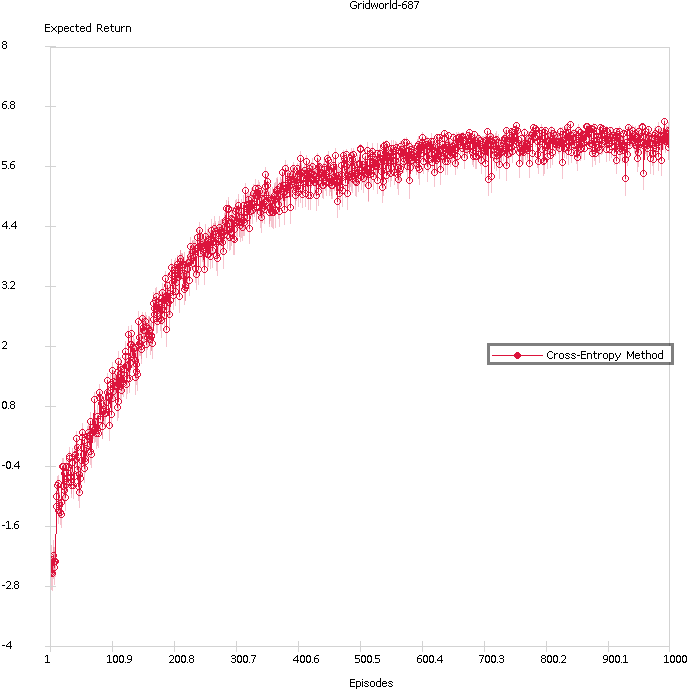
\includegraphics[scale=0.5]{Gridworld-687_18th_theBest}
\caption{GridWorld Plot}
\label{fig:grid}
\end{figure}


\begin{figure}
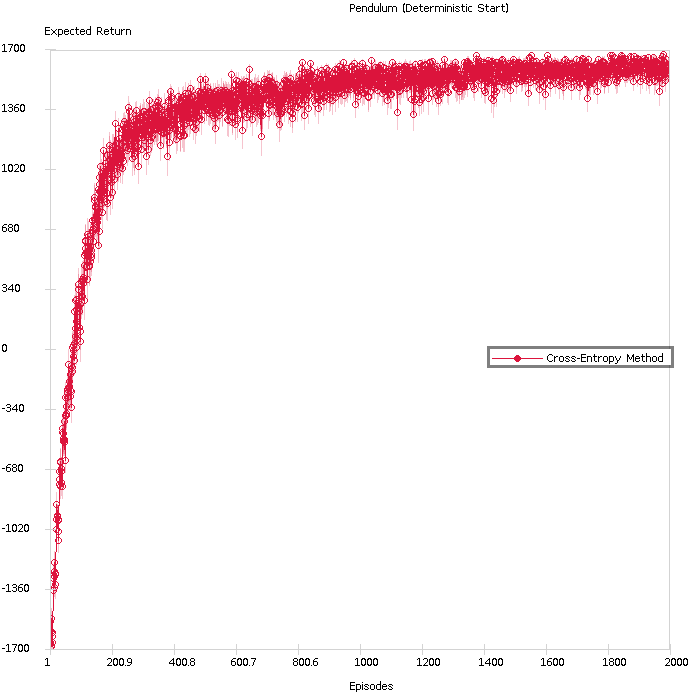
\includegraphics[scale=0.5]{Pendulum_Det}
\caption{pendulum-D Plot}
\label{fig:pendulum-D}
\end{figure}

\begin{figure}
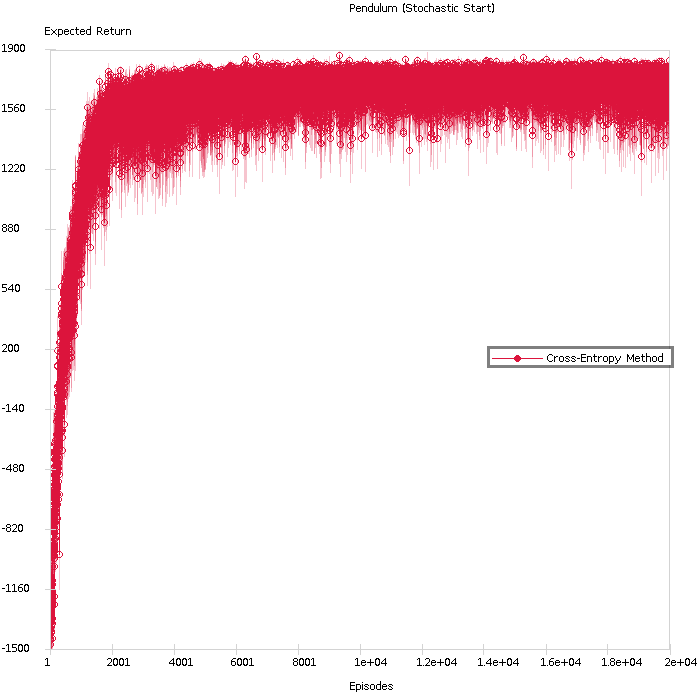
\includegraphics[scale=0.5]{Pendulum_Sto}
\caption{pendulum-S Plot}
\label{fig:pendulum-S}
\end{figure}

\end{document}

